
\documentclass[a4paper,12pt]{article}
\usepackage{amsmath, amssymb}
\usepackage{siunitx}
\usepackage{hyperref}
\usepackage{graphicx}
\usepackage{float}
\usepackage[a4paper, top=0.5in, bottom=0.5in, left=1in, right=1in]{geometry}
\usepackage{xcolor}
\usepackage{colortbl}
\usepackage{titlesec}
\usepackage{fontspec}
\usepackage{tikz}
\usepackage{lipsum} % For dummy text, remove this for your actual report
\usepackage{listings}
\usepackage{subcaption}
\lstset{
    language=Python,        % Specify the language
    basicstyle=\ttfamily,   % Basic font style
    keywordstyle=\color{blue}\bfseries, % Keywords style
    commentstyle=\color{green},         % Comments style
    stringstyle=\color{red},            % Strings style
    numbers=left,                      % Add line numbers
    numberstyle=\tiny,                 % Line number style
    stepnumber=1,                      % Step between line numbers
    frame=single,                      % Add a frame around the code
    breaklines=true                    % Allow breaking long lines
}
% Define colors
\definecolor{myblue}{rgb}{0.1, 0.2, 0.7}
\definecolor{mygreen}{rgb}{0.1, 0.6, 0.1}
\definecolor{myred}{rgb}{0.7, 0.2, 0.2}
\definecolor{lightblue}{rgb}{0.8, 0.9, 1}
\definecolor{mygold}{rgb}{0.8, 0.6, 0.1}
\definecolor{mygray}{rgb}{0.9, 0.9, 0.9}

% Customize title formatting
\titleformat{\title}[block]
  {\normalfont\Huge\bfseries\color{myblue}}{}{0em}{}

\titleformat{\author}[block]
  {\normalfont\LARGE\itshape\color{mygreen}}{}{0em}{}

% Custom header line
\newcommand{\myheader}{
    \noindent\rule{\textwidth}{1pt}\\[0.4cm]
}

% Title page design
\begin{document}

% Title Page
\begin{titlepage}
    \centering
    
    \vspace*{2cm}
    
    % Title
    {\Huge \bfseries \textcolor{myblue}{Lab Report:Bode Plot Analysis of RC Low-Pass Filters}}\\[0.5cm]
    {\LARGE \textit{\textcolor{myred}{Magnitude and Phase Response for 1st,2nd and 3rd Order}}\\[1.5cm]
    
    % Author names
    \noindent
    \textbf{\Huge Krishna Patil-EE24BTECH11036}\\[0.3cm]
    \textbf{\Huge Deepak Ahirwar-EE24BTECH11014}\\[1.5cm]
    
    % Institution name
    {\LARGE \textit{Electrical Department, IIT-Hyderabad}}\\[2cm]
    
    \vfill
    
    % Date
    {\LARGE \today}
    
    % Footer - with gradient line and custom footer text
    \vfill
    \myheader
    \centering
    \textcolor{mygold}{\Large \textit{Experiment conducted as part of ELectric Circuits Lab Coursework.}}
    
\end{titlepage}

\newpage


\section{\textcolor{myred}{INTRODUCTION}}
This lab investigates the frequency response of single-stage, two-stage, and three-stage RC low-pass filters using Bode plots. The study involves plotting magnitude and phase responses, deriving theoretical equations, and verifying experimental results using an oscilloscope and function generator.

\section{\textcolor{myred}{CIRCUIT DIAGRAMS}}
The circuit diagrams for the 1-stage, 2-stage, and 3-stage RC low-pass filters consist of cascaded resistor-capacitor networks.

\section{\textcolor{myred}{THEORETICAL ANALYSIS}}
The transfer function for a single-stage RC low-pass filter is given by:
\begin{equation}
H_1(j\omega) = \frac{1}{1 + j\omega RC}
\end{equation}
For a two-stage filter:
\begin{equation}
H_2(j\omega) = \left(\frac{1}{1 + j\omega RC}\right)^2
\end{equation}
For a three-stage filter:
\begin{equation}
H_3(j\omega) = \left(\frac{1}{1 + j\omega RC}\right)^3
\end{equation}

The magnitude response in decibels is:
\begin{equation}
|H_n(j\omega)|_{dB} = 20n \log_{10} \left(\frac{1}{\sqrt{1 + (\omega RC)^2}} \right)
\end{equation}

The phase response is:
\begin{equation}
\theta_n(\omega) = -n \tan^{-1}(\omega RC)
\end{equation}

\section{\textcolor{myred}{EXPERIMENTAL SETUP}}
\textbf{Equipment Used:}
\begin{itemize}
    \item Oscilloscope
    \item Function generator
    \item Resistors (2k$\Omega$)
    \item Capacitors (1000$\mu$F)
    \item Breadboard \& Connecting wires
\end{itemize}

\section{\textcolor{myred}{PROCEDURE TO OBTAIN READINGS}}
\begin{enumerate}
    \item Construct the RC circuit as per the circuit diagram.
    \item Connect the input of the circuit to a function generator and apply a sine wave signal.
    \item Use an oscilloscope to measure input and output voltages.
    \item Vary the frequency from 10Hz to 1MHz and note the amplitude and phase shift.
    \item Use the oscilloscope cursors to measure the phase difference between input and output waveforms.
\end{enumerate}

\section{\textcolor{myred}{Images of the readings}}


\begin{figure}[h]
    \centering
    \begin{minipage}{0.3\textwidth}
        \centering
        \includegraphics[width=\textwidth]{fig/Fig1 (1).jpg}
    \end{minipage}
    \begin{minipage}{0.3\textwidth}
        \centering
        \includegraphics[width=\textwidth]{fig/Fig1 (2).jpg}
    \end{minipage}
    \begin{minipage}{0.3\textwidth}
        \centering
        \includegraphics[width=\textwidth]{fig/Fig1 (3).jpg}
    \end{minipage}

    \begin{minipage}{0.3\textwidth}
        \centering
        \includegraphics[width=\textwidth]{fig/Fig1 (4).jpg}
    \end{minipage}
    \begin{minipage}{0.3\textwidth}
        \centering
        \includegraphics[width=\textwidth]{fig/Fig1 (5).jpg}
    \end{minipage}
    \begin{minipage}{0.3\textwidth}
        \centering
        \includegraphics[width=\textwidth]{fig/Fig1 (6).jpg}
    \end{minipage}

    \begin{minipage}{0.3\textwidth}
        \centering
        \includegraphics[width=\textwidth]{fig/Fig1 (7).jpg}
    \end{minipage}
    \begin{minipage}{0.3\textwidth}
        \centering
        \includegraphics[width=\textwidth]{fig/Fig1 (8).jpg}
    \end{minipage}
    \begin{minipage}{0.3\textwidth}
        \centering
        \includegraphics[width=\textwidth]{fig/Fig1 (9).jpg}
    \end{minipage}

    \begin{minipage}{0.3\textwidth}
        \centering
        \includegraphics[width=\textwidth]{fig/Fig1 (10).jpg}
    \end{minipage}
    \begin{minipage}{0.3\textwidth}
        \centering
        \includegraphics[width=\textwidth]{fig/Fig1 (11).jpg}
    \end{minipage}
    \begin{minipage}{0.3\textwidth}
        \centering
        \includegraphics[width=\textwidth]{fig/Fig1 (12).jpg}
    \end{minipage}

    \begin{minipage}{0.3\textwidth}
        \centering
        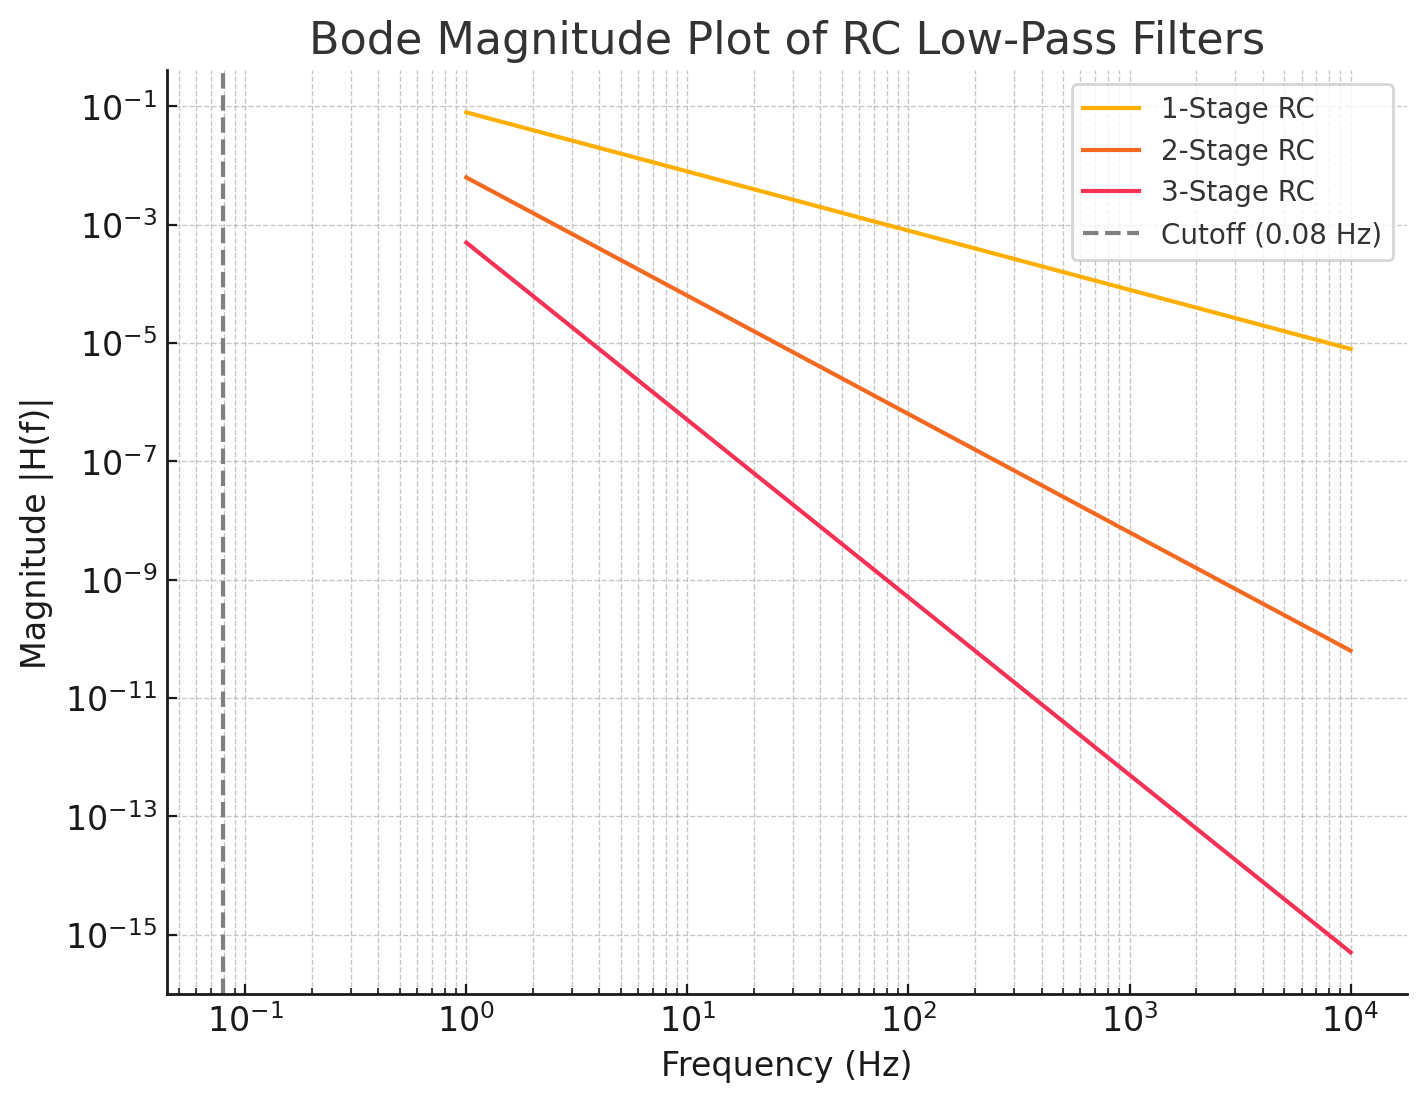
\includegraphics[width=\textwidth]{fig/plot.jpg}
    \end{minipage}

    \caption{Bode plots}
    \label{fig:13images}
\end{figure}



\section{\textcolor{myred}{CONCLUSION}}
The experiment successfully demonstrated the frequency-dependent behavior of RC low-pass filters. Higher-order filters provide sharper roll-off characteristics, making them more effective for noise filtering in signal processing applications.

\end{document}

